\chapter{Introduction}

\chapter{Problem Definiton}

%Some types of cancer are suspected to either originate in or else being influenced by genetic disposition. Though human DNA has been examined and broken down to sequences of genes the meaning of most genes and their influence on each other is still unknown. The Cerberus application enables doctors to get an overview over patients' gene-expression data as well as clinical data like the history of the disease. It uses clustering techniques to provide information visualization, thereby allowing doctors to systematically search for coincidences. The aim of this thesis is to extend the application with a metabolic pathway module to take the connection between metabolic pathways and genes into account. 

\chapter{Related Work}

In this chapter first...

\section{Metabolic Pathway Visualization}

\subsection{Medical Pathways}

\begin{figure}[ht]
\centering
\scalebox{0.43}{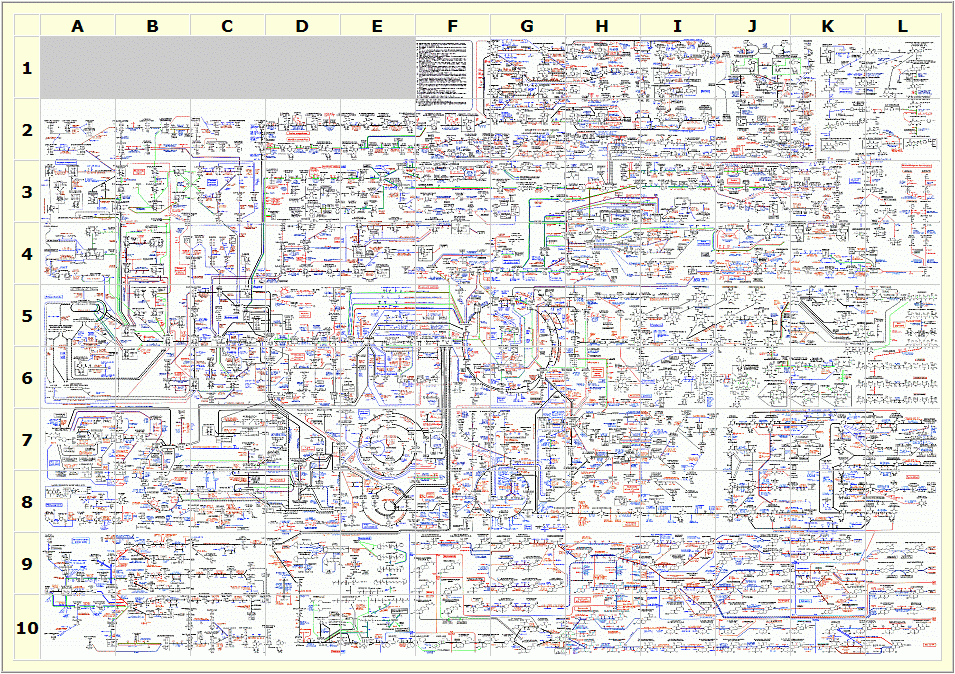
\includegraphics{gfx/RocheAppliedScience_MetabolicPathways_WallChart}} 
\caption[Roche Applied Science wall chart on metabolic pathways]{\textit{Roche Applied Science wall chart on metabolic pathways TODO Insert Reference}} 
\label{gfx:RocheAppliedScience_MetabolicPathways_WallChart}
\end{figure}

Metabolic pathways aim on modelling cellular functions in graphs. Basic building blocks of pathways are chemical compounds and enzymes. The chemical compounds act as substrates and products of chemical reactions. Enzymes catalyze these reactions by using substrates as input which is resulting in products. This process is described in LINK.

\subsection{State-of-the-art Frameworks}

\minisec{PathwayExplorer [2005]}

The PathwayExplorer is able to map genes on enzymes in pathways from various databases.
Positive: Can handle all kind of identifiers (for example RefSeq, ...).
Negative: Needs time to map genes on pathways. The result are static PNG images.

\begin{figure}[ht]
\centering
\scalebox{0.43}{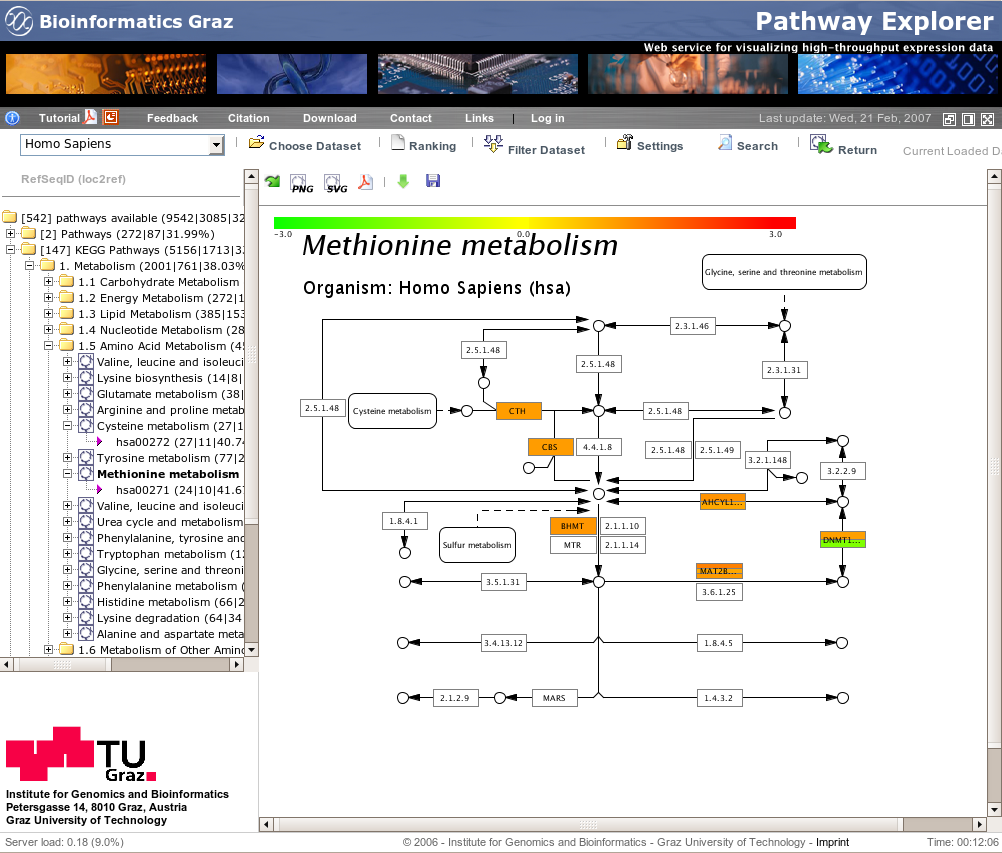
\includegraphics{gfx/screenshot_pathway_explorer}} 
\caption[PathwayExplorer]{\textit{PathwayExplorer}} 
\label{gfx:pathway_explorer}
\end{figure}

\section{Gene Expression Visualization}

\subsection{Gene-Expression Analysis}

Describe the Genome.
Human genome is sequenced since [year] by [name] -> Reference 
Describe how genes code enzymes (special proteins).
\subsection{State-of-the-art Frameworks}

http://www.genome.jp/kegg/expression/

\minisec{GeneSpring}
\minisec{Panther}

\section{Biomedical Databases}

Criterias for successful databases: 
Availability
Update rate / update process
ID Management (Unique Key)
Links to other databases
Software to access database (SOAP)
Documentation
Full data dump

\subsection{Gene centered databases}

\subsubsection{International Nucleotide Sequence Database Collaboration (INSDC)}

The INSDC is a collaborative network of DNA sequence databases that consists of three major members:
\begin{itemize}
 \item \textbf{GenBank:} \\
 GenBank is a part of the National Center for Biotechnology Information (NCBI) which is intergrated in the United States National Library of Medicine (NLM). NLM belongs to the National Institutes of Health (NIH) that is self-described as the focal point for medical research in the United States.
 \item \textbf{European Molecular Biology Laboratory (EMBL):} \\
 EMBL
 \item \textbf{DNA Data Bank of Japan (DDBJ)} \\
\end{itemize}

INSERT table with current data sets in various databases
Number of genes, proteins, enzymes.

\subsubsection{Entrez}

\subsubsection{Gene Ontology (GO)}

\subsection{Pathway centered databases}

\subsubsection{Kyoto Encyclopedia of Genes and Genomes (KEGG)}

The Kyoto Encyclopedia of Genes and Genomes (KEGG)\footnote{http://www.genome.jp/kegg/} is a biomedical resource that started its online service in 1995 and belongs to the Japanese GenomeNet.

Provide pathways for over ?? organisms.

In the graph enzymes are visualized by rectangular nodes and compounds are modelled by small circles. Round rectangular nodes depict linked pathways. This circumstance points to the fact that a pathway is only an artificial subset of a huge complex network. 


When a cellular function is valid throughout different organisms it is called strongly preserved. These general pathways are stored in the KEGG database as reference pathways. Each reference pathway can then be specialized for a specific organism. Figure BLA shows the methionine metabolism for home sapiens. Light green color coded enzymes depict proteins where the generating genes are known. 

\begin{figure}[ht]
\centering
\scalebox{0.4}{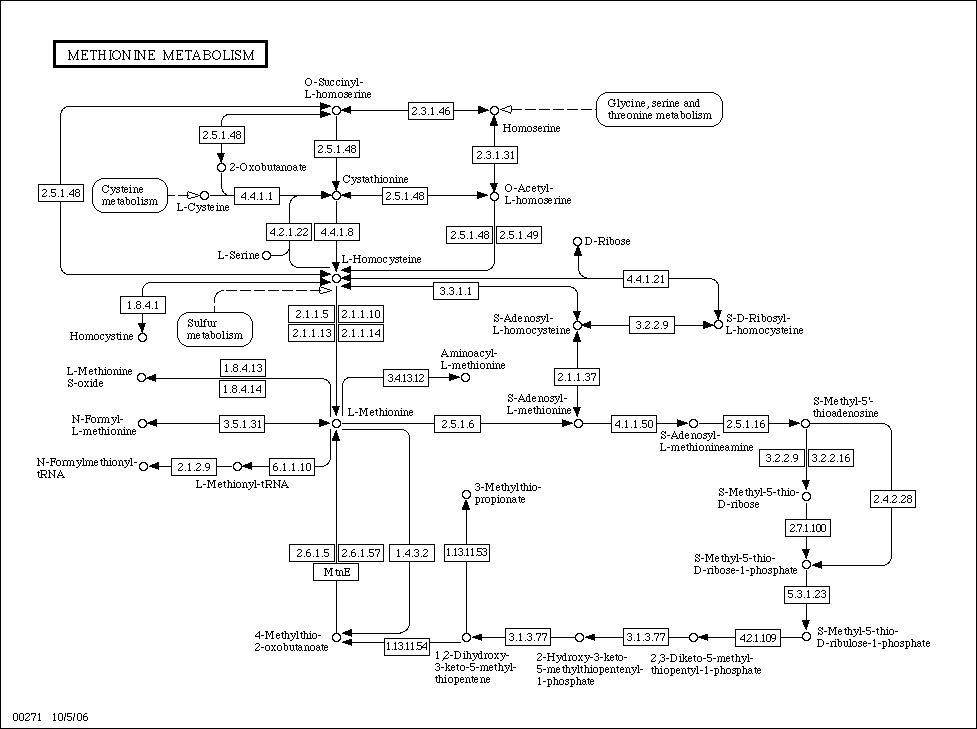
\includegraphics{gfx/KEGG_methionine_metabolism_271_reference_pathway}} 
\caption[KEGG methionine metabolism reference pathway]{\textit{KEGG methionine metabolism reference pathway}} 
\label{gfx:KEGG_methionine_metabolism_271_reference_pathway}
\end{figure}

\begin{figure}[ht]
\centering
\scalebox{0.4}{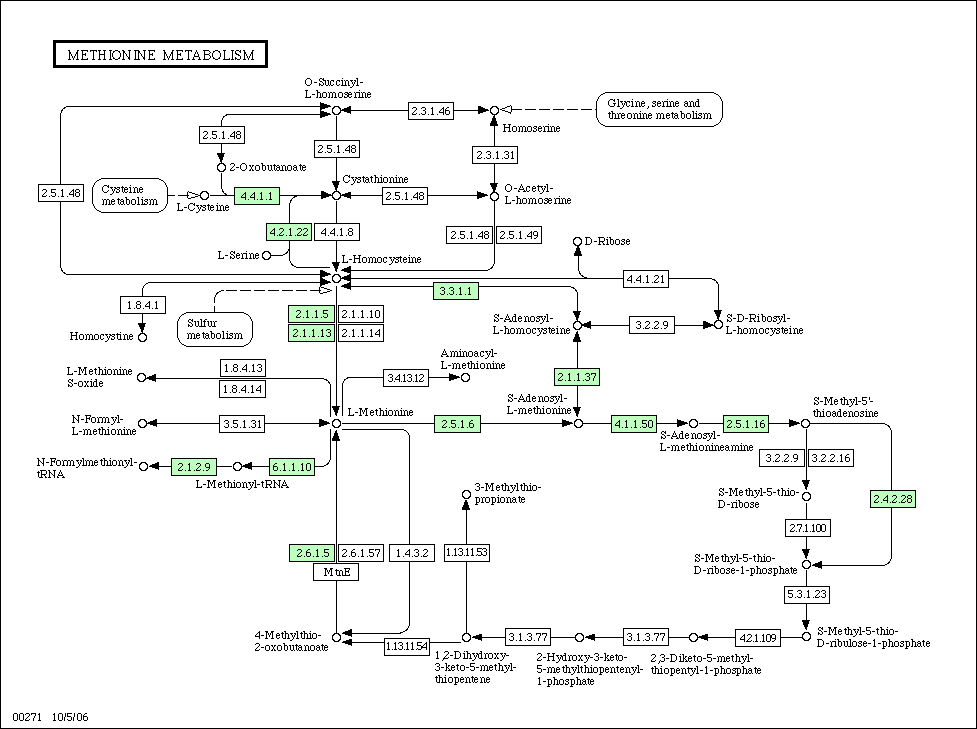
\includegraphics{gfx/KEGG_methionine_metabolism_271_pathway_hsa}} 
\caption[KEGG methionine metabolism pathway for home sapiens]{\textit{KEGG methionine metabolism pathway for home sapiens}} 
\label{gfx:KEGG_methionine_metabolism_271_pathway_hsa}
\end{figure}

\subsection{Biomedical Identification Numbers}

During the last decade biochemical database projects sprang up like mushrooms. Some projects has proven their value and achieved to manifest themeselves inside the community. Each database project introduced their own identification numbers for genes, proteins, nucleotids, etc. The obvious problem is how to map these data and interconnect them among the misscellaneous databases. 
There were many attempts over the time to get the issue under control.

The nomenclature for enzymes become widely accepted. The Nomenclature Committee of the International Union of Biochemistry and Molecular Biology (NC-IUBMB) agreed on the Enzyme Commission number (EC number). For details see http://www.chem.qmul.ac.uk/iubmb/enzyme/.

In the case of genes unique identifiers are much more silvered.

Identification Number

\section{Information Visualization Methods}

\subsection{2D vs. 3D}

\subsection{Multiple Views}
\subsection{Focus + Context}
\subsection{Linking \& Brushing}
\subsection{Semantic Zooom}

\section{Application of Gene-Expression Data onto Metabolic Pathways}



%Nochmal in implementation/results

\chapter{System Architecture}

\section{Overall Design}
%\section{Data Management}
\section{Pathway Data Management}

From information point of view metablic pathways are graphs. The nodes are enzymes and compounds. The edges can be differenciated in relations and reactions.


Show relations between data (1:1, 1:n, etc).
%\subsection{Set / Storage / Virtual Array}

%Referenz auf Michaels Thesis

\section{Graphical User Interface (GUI)}

\section{Data Update Mechanism}

%Selection handling included 

\chapter{Implementation}

\section{Used Technologies}
\subsection{SWT}

%SWT successor of AWT.
%Abstract Widget Toolkit (AWT)

\subsection{JOGL}

%Java OpenGL library\footnote{https://jogl.dev.java.net/}

%\subsection{OpenGL integration in Java}
\subsection{JGraph}

\section{Data Loading}

\section{Visualization Techniques}

\subsection{2D Pathway Implementation}
\subsubsection{Pathway Switching}
\subsubsection{Hierarchical Pathways}

\subsubsection{Neighborhood Visualization}


In graphs where the layout aims on the positioning of nodes and edges to circumvent intersections neighborhood visualization takes an important role. 
Cyclic charakter


Modified Breadth-First-Search (BFS) Algorithm.

\subsection{OpenGL Pathways}
\subsubsection{Pathway Texture Overlay}
\subsubsection{Pathway Linking}
\subsubsection{Pathway Element Picking}
\subsubsection{Hierarchical Display Lists}
\subsubsection{Layered Pathways}
\subsubsection{Panel View}

\chapter{Results}

%Reflections from Zatloukal

\chapter{Conclusions}

\chapter{Future Work}

\index{bla}


